При достаточно высокой энергии гамма-кванта наряду с фотоэффектом и эффектом
Комптона может происходить третий вид взаимодействия гамма-квантов с веществом –
образование электрон-позитронных пар. Процесс образования пар не может
происходить в пустоте, так как в этом случае не выполняются законы сохранения
энергии и импульса. В присутствии ядра или электрона процесс образования пары
гамма-квантом возможен, так как можно распределить энергию и импульс
гамма-кванта между тремя частицами без противоречия с законами сохранения. При
этом если процесс образования пары идет в кулоновском поле ядра или протона, то
энергия образующегося ядра отдачи оказывается весьма малой, так что пороговая
энергия гамма-кванта $E_0$, необходимая для образования пары, практически
совпадает с удвоенной энергией покоя электрона $Е0 \approx 2 m c^22 = 1,022$
МэВ. Появившийся в результате процесса образования пар электрон теряет свою
энергию на ионизацию среды. Таким образом, вся энергия электрона остается в
детекторе. Позитрон будет двигаться до тех пор, пока практически не остановится,
а затем аннигилирует с электроном среды, в результате чего появятся два
гамма-кванта. Т.е., кинетическая энергия позитрона также останется в детекторе.
Далее возможны три варианта развития событий: а) оба родившихся гамма-кванта не
вылетают из детектора, и тогда вся энергия первичного гамма-кванта останется в
детекторе, а в спектре появится пик с $Е = Е_{\gamma}$; б) один из родившихся
гамма-квантов покидает детектор, и в спектре появляется пик, соответствующий
энергии $Е = Е_{\gamma} - E_0$, где $Е_0= m c^2 = 511$ кэВ; в) оба родившихся
гамма-кванта покидают детектор, и в спектре появляется пик, соответствующий
энергии $Е = Е_{\gamma} - 2 E_0$, где $2 Е_0 = 2 m c^2 = 1022$ кэВ. Таким
образом, любой спектр, получаемый с помощью гаммаспектрометра, описывается
несколькими компонентами, каждая из которых связана с определенным физическим
процессом. Как описано выше, основными физическими процессами взаимодействия
гамма-квантов с веществом являются фотоэффект, эффект Комптона и образование
электронпозитронных пар, и каждый из них вносит свой вклад в образование
спектра. Помимо этих процессов, добавляются экспонента, связанная с наличием
фона, пик характеристического излучения, возникающий при взаимодействии
гамма-квантов с окружающим веществом, а также пик обратного рассеяния,
образующийся при энергии квантов $Е_{\gamma} \gg m c^2 / 2$ в результате
рассеяния гамма-квантов на большие углы на материалах конструктивных элементов
детектора и защиты. Положение пика обратного рассеяния определяется по формуле:

\begin{equation}
  E_{\text{обр}} = \frac{E}{1 + \frac{2 E}{m c^2}}
\end{equation}

где $Е$ – энергия фотопика, На рис.1 приведен в качестве примера спектр,
полученный при регистрации сцинтилляционным гамма-спектрометром гамма-квантов,
излучаемых радиоактивными ${}^{60}{\text{Co}}$.

\begin{figure}[h!]
  \centering
  \includegraphics[width=0.8\linewidth]{pic1.png}
  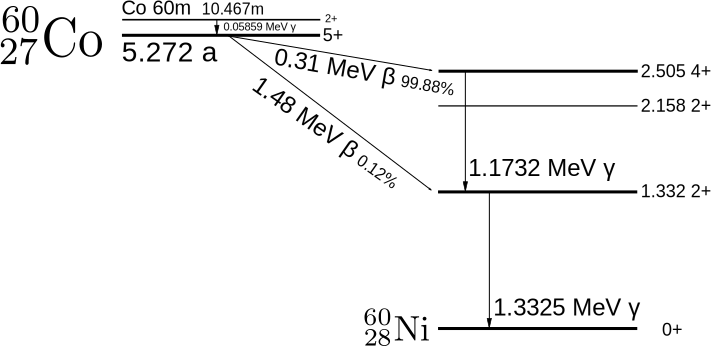
\includegraphics[width=0.6\linewidth]{pic2.pdf}
  \caption{Спектр ${}^{60}{\text{Co}}$ и схема его распада}
  \label{pic:Cobalt}
\end{figure}

При бета-распаде ${}^{60}{\text{Co}}$. образуется радиоактивный
${}^{60}{\text{Ni}}$. в возбужденных состояниях с энергиями $2,505$ МэВ либо
$1,332$ МэВ. Распад высокоэнергетичного состояния происходит преимущественно на
первый возбужденный уровень и при этом испускается гамма-квант с энергией
$1,173$ МэВ. На этом рисунке видны два фотопика, соответствующие этим квантам.
Кроме того, наблюдается непрерывное комптоновское излучение, пик обратного
рассеяния и характеристическое излучение из свинца, служащего защитой детектора
от космического излучения. На рис. 2 приведен еще один спектр,
зарегистрированный от радиоактивного изотопа ${}^{137}{\text{Cs}}$, который
является источником гамма-квантов с энергией $661,7$ кэВ. На этом спектре
сплошными линиями показаны пик полного поглощения, обусловленный фотоэффектом,
пик характеристического излучения, пик обратного рассеяния, и экспоненциальный
фон. На рис. 3 приведен спектр, полученный от радиоактивного изотопа
${}^{22}{\text{Na}}$. Источник ${}^{22}{\text{Na}}$ кроме $\gamma$-излучения
испускает позитроны, которые при аннигиляции с электронами дают в спектре резкий
аннигиляционный пик, соответствующий энергии $511$ кэВ. В спектре этого
источника есть также гамма-кванты с энергией $1,275$ МэВ.
